\documentclass[a4paper, 1.5lines]{ctexart}
\usepackage[top=3cm, bottom=2cm]{geometry}
\usepackage{graphicx}
\usepackage{subcaption}
\usepackage{amsmath}
\usepackage{amssymb}
\usepackage{amsfonts}
\usepackage{xcolor}
\usepackage{booktabs}
\usepackage{url}
\usepackage{pdfpages}
\usepackage{multirow}
%\usepackage{hyperref}
\usepackage[hidelinks]{hyperref} % 加载 hyperref 并隐藏链接边框
\usepackage{fancyhdr} % 导入fancyhdr宏包
\usepackage{lipsum} 


%\usepackage[utf8]{inputenc}
%\usepackage[ngerman]{babel} % 加载德语支持

% booktabs 提供 \toprule, \midrule, \bottomrule 等表格命令
\usepackage{booktabs}
% 定义占位命令以避免未定义控制序列错误
\newcommand{\placeholderspace}{}
\usepackage{fancyhdr} % 导入fancyhdr宏包
\usepackage{lipsum}   % 仅用于生成示例文本
\usepackage{float}    % 提供 H 浮动位置选项

% 设置页面样式为fancy
\pagestyle{fancy}
% 自定义页眉内容
\fancyhead[L]{} % 左侧页眉
\fancyhead[C]{\textbf{Physics-experiment Reporting Letter:\\Physical Properties of Liquid Crystals}} % 中间页眉
\fancyhead[R]{ } % 右侧页眉
% 自定义页脚内容
\fancyfoot[L]{ } % 左侧页脚
\fancyfoot[C]{\thepage} % 中间页脚显示页码
\fancyfoot[R]{ } % 右侧页脚
% 改变页眉线的粗细
\renewcommand{\headrulewidth}{1.4pt}
% 改变页脚线的粗细
\renewcommand{\footrulewidth}{0.pt}

\title{液晶物性}
\author{实验人：唐亿\qquad 学号：202311998381\qquad 指导教师：陈荣艳}
\date{实验日期：2026.1.9}


\begin{document}
    
    \maketitle
            
    \begin{abstract}
         本实验围绕向列相液晶盒的物理特性展开研究，重点考察其光学各向异性行为以及在外加电场作用下的电光响应。实验内容包括液晶材料双折射与旋光特性的表征，并系统测量了不同驱动电压条件下的透射光强变化规律，从而获得其电光响应曲线及响应时间特性。实验采用常黑工作模式，通过调节施加于液晶盒两端的电压，研究电场对出射光强的调制效应。同时，对液晶材料的上升沿与下降沿响应时间进行了测量。最后，通过对实验中出现的衍射现象进行分析，对液晶体系所形成的等效光栅结构参数进行了估算。
        
        \textbf{\textbf{关键词：液晶物性、双折射、电光响应、Williams 畴}}
    \end{abstract}
    
    \section{引言}
        许多有机化合物在受热过程中会经历一种介于固态与各向同性液态之间的特殊相态。当温度升高至熔点附近时，这类物质首先转变为呈现浑浊外观的液体；继续升温至清亮点后，体系会突然变为光学性质各向同性的透明液体。在熔点与清亮点之间存在的这一中间相，既保持了液体的流动性，又表现出显著的各向异性特征，被称为液晶相。正是由于液晶在电、光及磁等方面所展现出的多样而独特的各向异性行为，使其成为凝聚态物理与材料科学中长期关注的研究对象，并在技术发展推动下逐步应用于显示器件等实际产品中。

本实验以向列相液晶盒为研究对象，对其典型物理性质进行系统考察。液晶材料本身作为各向异性光学介质，会对通过其中的光产生双折射效应；而液晶盒通过对液晶分子的定向排列与扭转结构设计，使体系进一步表现出旋光特性。这两种效应均会导致入射光偏振态的改变。在外加电场作用下，液晶分子的取向将随电压变化而发生调整，从而引发明显的电光响应。实验中将围绕液晶盒的电光调制行为展开研究，重点分析其响应特性、时间行为以及在特定条件下出现的衍射现象。
    \section{原理}
       液晶态并非物质普遍具有的相态，其性质区别于常见的固态、液态和气态。一般而言，只有分子尺度较大且形状具有明显各向异性的物质才可能形成液晶相，其中最典型的是分子呈杆状或碟状结构、轴向与横向尺寸比约为 $4{:}1$ 至 $8{:}1$ 的体系。对于由杆状分子构成的液晶体系，其液晶相可依据分子在空间中的平移有序性与取向有序性进行分类，主要包括近晶相、向列相和胆甾相三种类型。本实验所研究的液晶盒属于向列相液晶体系。

       \subsection{液晶的光学各向异性——双折射效应}
        当光入射到各向异性晶体中时，由于介质对不同偏振方向的响应不同，光将分解为两种传播性质不同的分量。若光的偏振方向垂直于晶体的光轴，其对应的折射率为普通光折射率 $n_{\mathrm{o}}$，该分量满足通常的折射定律；而当光的偏振方向平行于光轴时，其折射率为非常光折射率 $n_{\mathrm{e}}$，传播方向一般不再严格遵循折射定律。

对于偏振方向与光轴成 $\theta$ 角入射的线偏振光，可将其视为沿上述两种本征偏振方向的叠加。由于两种分量在晶体中具有不同的折射率，它们在传播过程中将积累不同的光程，从而在出射时产生相位差
\begin{equation}
    \delta = \dfrac{2\pi}{\lambda}(n_{\mathrm{o}} - n_{\mathrm{e}}) d ,
\end{equation}
其中 $\lambda$ 为入射光波长，$d$ 表示光在晶体中传播的有效厚度。

线偏振光通过液晶盒后，正是由于这种双折射效应，其偏振态会发生改变。通过调节液晶盒的有效厚度 $d$，可以控制相位差的大小，从而实现对出射光偏振状态的调制。

在特定条件下，出射光的偏振形式具有明确的判据。当相位差满足 $\delta = \pi/2$ 时，若入射偏振方向与光轴取特定角度关系，则出射光可能保持为线偏振光；在另一类取向条件下，出射光将转化为圆偏振光，其余情形对应椭圆偏振光。当相位差为 $\delta = \pi$ 时，出射光仍为线偏振光，但其偏振方向相对于入射光将关于光轴发生对称翻转。
        \subsection{液晶盒结构及其旋光性}
        实验中所使用的液晶为向列相液晶。在该相态下，液晶分子在空间中整体呈现出取向上的平行有序，而分子重心的位置分布则仍保持无序状态。因此，向列相液晶通常主要表现出光学各向异性，其最典型的性质为双折射效应，而本身并不具有显著的旋光性。

当液晶层被限制在两个基片之间，并通过表面处理使上下基片处的分子取向方向发生均匀扭转时，便可制成具有旋光特性的液晶盒。此时，液晶体系对左旋光和右旋光的折射率不再相同，导致入射线偏振光在传播过程中偏振面的连续旋转，从宏观上表现为旋光效应。一般而言，旋转角度 $\theta$ 与光在介质中传播的厚度 $d$ 成正比关系。

实际应用中，液晶材料通常被封装在两片镀有透明导电薄膜的玻璃基片之间。基片表面经过定向处理后，会对邻近液晶分子的取向产生约束作用，从而使整个液晶层形成稳定的取向结构，这种器件称为液晶盒。对于扭曲向列相（Twisted Nematic, TN）液晶盒，上下基片处液晶分子的取向方向相互垂直，液晶分子沿厚度方向发生均匀扭转，总体旋转角度约为 $90^\circ$，因此该结构表现出较强的旋光特性。

当线偏振光通过具有旋光性的介质后，其振动方向将发生旋转，旋转角度 $\beta$ 与旋光物质的厚度 $d$ 满足
\begin{equation}
    \beta = \alpha(\lambda)\, d ,
\end{equation}
其中 $\alpha(\lambda)$ 为旋光本领（或称旋光率），其数值与入射光波长 $\lambda$ 有关。
\subsection{液晶的电光效应}

液晶的电光效应是指在外加电场作用下，液晶分子的取向结构发生重新排列，从而引起液晶盒整体光学性质变化的一种电控光学调制现象。由于液晶材料具有明显的介电各向异性，外电场会对分子取向产生定向力矩，使原有的取向结构发生畸变或重排，进而改变其对偏振光的调制特性。

\subsubsection{电光响应曲线}

在外加电场作用下，液晶分子的取向状态会随电压变化而逐渐偏离原有的稳定结构。具体到液晶盒中，这一过程表现为随着施加电压的增大，液晶分子原先的扭曲排列逐步被破坏。为便于定量研究这一效应，实验中固定入射光的偏振方向以及出射端检偏器的位置，仅将液晶盒上的驱动电压作为变量进行调制。

实验采用“常黑模式”进行观测，即在未加电压时，入射到液晶盒中的线偏振光经液晶盒后仍保持偏振态，并在检偏器处处于消光状态。此时，液晶盒光学性质的任何改变都会直接反映为检偏器后出射光强偏离消光条件的程度。

实验中主要测量两个物理量：一是由函数发生器提供的驱动电压 $U(t)$，二是经检偏器后输出的光强信号 $I(t)$，后者通过响应速度较高的光电二极管进行探测。两路信号分别接入示波器的 CH$_1$ 和 CH$_2$ 通道，由此可以得到光强 $I$ 随电压 $U$ 变化的关系曲线，即液晶盒的电光响应曲线。该曲线通常表现出明显的阈值特性：当电压超过某一临界值后，液晶盒的旋光结构被显著破坏，出射光强迅速增大。基于此，可引入阈值电压（光强达到最大值的 $0.1$ 处）、饱和电压（光强达到最大值的 $0.9$ 处）以及阈值锐度（饱和电压与阈值电压之比）等参数，用于表征液晶的电光响应特性。

\subsubsection{电光响应时间}

当施加在液晶盒上的电压发生变化时，液晶分子并不会瞬时达到新的平衡取向，而是需要经历一定的弛豫过程，这一时间尺度即为液晶的电光响应时间。为测量该响应过程，实验中对液晶盒施加周期性变化的高、低电平电压信号。在高电平阶段，为避免直流电场对液晶材料造成老化损伤，通常采用叠加高频脉冲的方式进行驱动。

因此，实验涉及的主要参数包括驱动电压幅值、高电平脉冲的频率以及高低电平交替的开关频率。由于电压上升和下降过程中液晶分子取向演化的动力学过程并不对称，上升过程与下降过程对应的响应时间也存在差异。实验中分别定义上升沿时间 $T_{\text{on}}$，即光强透过率由最小值上升至最大值的 $0.9$ 所需的时间，以及下降沿时间 $T_{\text{off}}$，即光强透过率由最大值下降至最大值的 $0.1$ 所需的时间，用以刻画液晶电光响应的动态特性。

\subsubsection{液晶衍射}

当施加在液晶盒上的低频电压超过某一临界值后，液晶中存在的带电杂质在电场驱动下发生迁移，进而诱发液晶分子的局域环流结构。这些微观环流在空间上呈现出周期性的分布，使液晶盒内部的分子取向发生规则性调制，从而形成折射率的周期变化结构。透过液晶盒的光在这种周期性介质中发生衍射，在屏幕上表现为明暗相间的条纹结构，称为 Williams 畴，其本质相当于一个光学衍射光栅。

在近似条件下，衍射环的数目 $N$ 与液晶材料的双折射率 $\Delta n$、液晶层厚度 $d$ 以及入射光波长 $\lambda$ 之间满足关系
\begin{equation}
    N \simeq \frac{\Delta n}{\lambda}\, d .
\end{equation}
该液晶所形成的位相型光栅同样满足一般光栅方程
\begin{equation}
    a \sin\theta = k \lambda ,
\end{equation}
其中 $a$ 为等效光栅常数，$\theta$ 为衍射角，$k$ 为衍射级次。

\section{实验}

\begin{itemize}
    \item \textbf{液晶旋光与双折射现象的观测}
    \begin{enumerate}
        \item 首先调节光路中的起偏器方向，使入射到液晶位置处的光强达到最大。随后转动检偏器，在未放置液晶盒的情况下测量出射光的线偏振特性，并记录光强取得极大值与极小值时检偏器对应的角度 $\theta_1$。
        \item 在起偏器与检偏器之间插入液晶盒，保持起偏器方向不变，缓慢旋转液晶盒，直至出射光再次呈现线偏振状态，即出现二次消光现象。此时，入射液晶盒的偏振光方向与液晶光轴平行或垂直。在该条件下，将检偏器旋转一周，记录两次光强极大和两次极小对应的角度 $\theta_2$。由于入射偏振方向已固定，且出射光为线偏振光，可通过角度差 $|\theta_1-\theta_2|$ 计算液晶盒的旋光角 $\beta$。
        \item 在二次消光的基础上，进一步旋转液晶盒，记录出射光强极大值与极小值对应的检偏器角度。结合旋转液晶盒前后偏振态的变化情况，可分析得到液晶盒引入的附加相位差 $\delta$，从而研究其双折射特性。
    \end{enumerate}

    \item \textbf{液晶的电光响应曲线测量}
    \begin{enumerate}
        \item 将实验系统调节至常黑模式，即在未加外电场时，检偏器后无光输出。随后设置函数发生器输出幅值约为 12\,V 的三角波信号，此时可观察到在电压线性上升和下降过程中液晶盒的电光响应行为。通过改变驱动信号的频率，还可以观察到电光响应曲线中可能出现的“磁滞回线”现象。
        \item 为获得较为准确的电光响应参数，如阈值电压、饱和电压以及阈值锐度，应选取频率较低的驱动信号进行测量，以减小动态效应对结果的影响。
    \end{enumerate}

    \item \textbf{液晶的电光响应时间测量}
    \begin{enumerate}
        \item 将原有光电池替换为响应速度更快的光电二极管，并接入约 12\,V 的工作电源。将液晶驱动电压设置在 12\,V 左右，通过旋转检偏器和液晶盒，使系统输出光强达到最小。在此条件下，利用示波器同时观察液晶的驱动信号与光学响应信号。
        \item 将驱动电源切换至间歇工作模式，分别调节间歇频率（开关频率）和驱动频率（脉冲频率），比较液晶响应信号随参数变化的特征。在选定的间歇频率条件下，测量液晶在电压上升与下降过程中的上升沿时间和下降沿时间。
    \end{enumerate}

    \item \textbf{液晶衍射现象与光栅常数估计}

    移除光探测器，在光路末端放置白屏用于直接观察衍射图样。缓慢增大施加在液晶盒上的调制电压，直至约 12\,V，记录衍射条纹首次出现和最终消失时对应的电压值；随后缓慢降低调制电压，同样记录衍射条纹出现和消失的电压范围。通过测量屏幕上相邻衍射光斑之间的间距，可对液晶形成的等效光栅常数进行估算。
\end{itemize}

\section{结果与分析讨论}

\subsection{无液晶时出射光的线偏度}

在实验开始前，由于实验环境中存在背景光强，需要首先对光电探测系统进行调零处理。随后测得入射光光强为
\[
I_{\text{in}} = 1.507\,\mathrm{mW}.
\]

在光路中加入起偏器并旋转一周，可以观察到出射光强随角度变化呈现周期性变化，在一周内出现两次极大值和两次极小值。

随后加入检偏器，并将起偏器固定在光强极大对应的位置。旋转检偏器一周后，同样可以观察到明显的消光现象，其对应的最大与最小输出光强分别为
\[
I_{\max} = 1.505\,\mathrm{mW}, \qquad
I_{\min} = 0.56\,\mathrm{\mu W}.
\]

由此可定义系统在无液晶条件下的线偏度
\begin{equation*}
L_0 = \frac{I_{\max}}{I_{\min}} = 2687.5.
\end{equation*}

\subsubsection{加入液晶之后出射光的偏振特性}

在光路中引入液晶盒后，通过旋转检偏器可以观察到多个消光位置。实验中测得若干次消光对应的检偏器角度分别为
\[
\theta_1 = -8.5^{\circ}, \quad
\theta_2 = 74.5^{\circ}.
\]

由相邻消光位置之间的角度差可以计算液晶引起的旋光角
\[
\theta = \theta_2 - \theta_1 = 83^{\circ},
\]
并利用第三次消光位置进行一致性检验。

随后以液晶盒的角度零点为参考，连续转动液晶盒，记录出射光强。实验结果表明，出射光强随液晶盒转角呈现周期性变化。

进一步在不同液晶盒转角处测量出射光强的极大值与极小值，其对应数值分别为
\[
I_{\max}(\phi_i) , \qquad
I_{\min}(\phi_i) .
\]
由此计算线偏度
\[
L(\phi_i) = \frac{I_{\max}(\phi_i)}{I_{\min}(\phi_i)} .
\]

\begin{table}[h!]
    \centering
    \caption{最小输出光强极值随液晶盒转角的变化}
    \label{key}
    \begin{tabular}{ccccccccc}
        \toprule
        液晶盒转角/$^\circ$ 
        & 34 & 83 & 125 & 170 & 218 & 257 & 305 & 351 \\
        \midrule
        光强极小值/$\mu$W 
        & 0.6 & 12.8 & 0.4 & 13.4 & 0.5 & 10.5 & 0.6 & 13.8 \\
        光强极大值/$\mu$W 
        & 858 & 841 & 869 & 815 & 844 & 859 & 851 & 806 \\
        线偏度 
        & 1430.0 & 65.7 & 2172.5 & 60.8 
        & 1688.0 & 81.8 & 1418.3 & 58.4 \\
        \bottomrule
    \end{tabular}
\end{table}
结果显示，线偏度随液晶盒转角呈现明显的周期性变化，反映了液晶取向对出射光偏振态的调制作用。


    \begin{figure}[h!]
        \centering
        \begin{subfigure}{0.47\textwidth}
            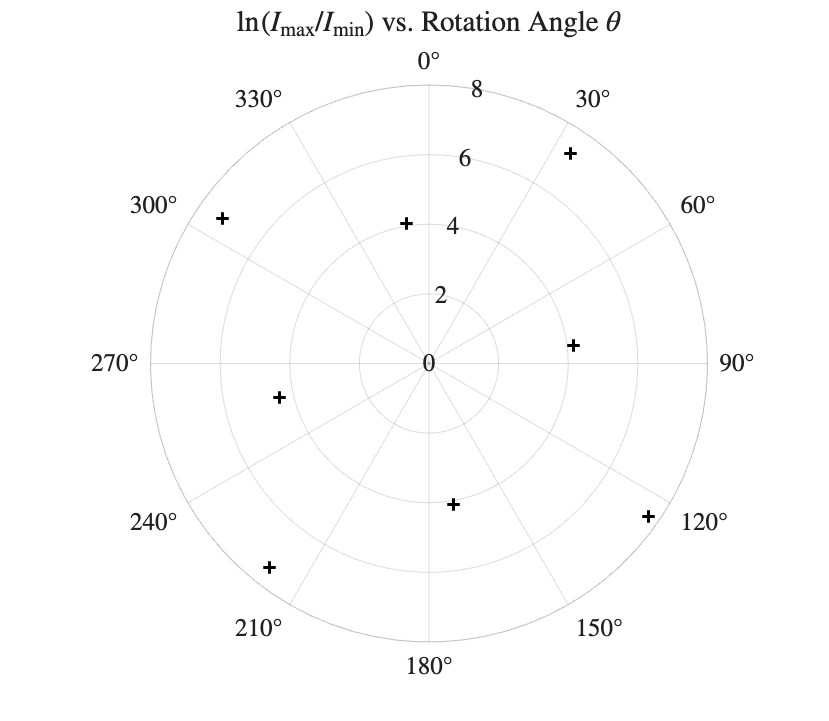
\includegraphics[width=7cm,height=6cm]{logratio.jpg}
            \caption{极值处线偏度的对数极坐标图}
            \label{key}
        \end{subfigure}
        \hfill
        \begin{subfigure}{0.47\textwidth}
            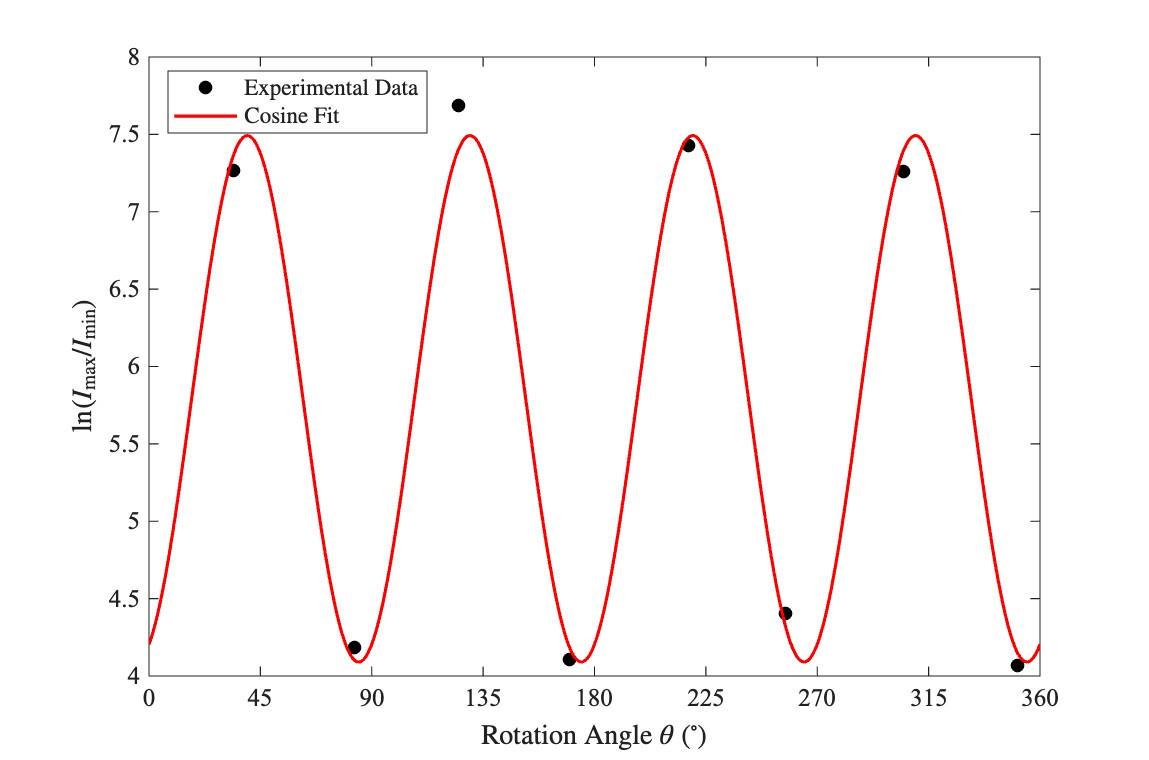
\includegraphics[width=8cm,height=5cm]{cosfit.jpg}
            \caption{线偏振度与角度的三角拟合}
            \label{key}
        \end{subfigure}
        \caption{最小输出光强及其线偏振度}
        \label{key}
    \end{figure}

\subsection{电光响应曲线}

将液晶调整至常黑工作模式后，使用函数发生器施加幅值为
\[
V_{\text{drive}} = 11.6\,\mathrm{V}
\]
的周期性驱动电压。在合适的驱动频率
\[
f = 1.992\,\mathrm{Hz}
\]
下，可以测得液晶的电光响应曲线，并观察到明显的磁滞回线现象。

通过对电光响应曲线进行数值拟合分析，可以得到液晶的阈值电压、饱和电压以及阈值锐度等参数，其结果分别为
\begin{table}[h!]
    \centering
    \caption{液晶电光响应曲线的阈值与锐度}
    \label{tab:electrooptic}
    \begin{tabular}{lccc}
        \toprule
        & 阈值电压/V & 饱和电压/V & 阈值锐度 \\
        \midrule
        下降 & 9.36 & 7.2  & 1.30 \\
        上升 & 9.60 & 8.88 & 1.08 \\
        \bottomrule
    \end{tabular}
\end{table}

在电压上升与下降过程中，上述参数存在一定差异，体现了液晶体系固有的磁滞特性。

 \begin{figure}[h!]
        \centering
        \begin{subfigure}{0.47\textwidth}
            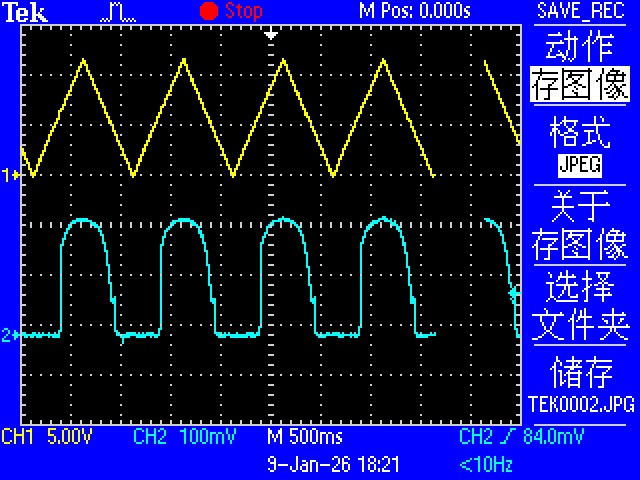
\includegraphics[width=\textwidth,height=6cm]{resp}
            \caption{电光响应曲线}
            \label{key}
        \end{subfigure}
        \hfill
        \begin{subfigure}{0.47\textwidth}
            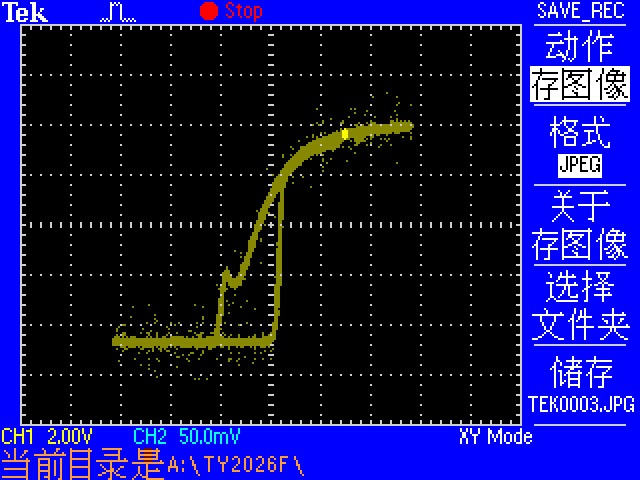
\includegraphics[width=\textwidth,height=6cm]{counter}
            \caption{磁滞回线}
            \label{key}
        \end{subfigure}
        \caption{常黑模式的电光响应曲线}
        \label{key}
    \end{figure}

\subsection{电光响应时间}

在保持液晶工作模式不变的条件下，使用函数发生器输出脉冲方波信号，调节驱动电压、驱动频率及开关频率，观察出射光强随时间的动态变化。

通过对响应曲线的上升沿与下降沿进行拟合分析，可以分别得到液晶的电光响应时间
\[
T_{\text{on}} = 11.6\,\mathrm{ms}, \qquad
T_{\text{off}} = 10.1\,\mathrm{ms}.
\]

实验结果表明，液晶的动态响应特性对驱动条件具有显著依赖性。

\subsection{液晶衍射与光栅常数估计}

在逐渐增加液晶调制电压的过程中，当电压达到
\[
V_{\text{diff}} = 8.74\,\mathrm{V}
\]
时，可以观察到明显的衍射图样出现。

在衍射图样较为稳定的条件下，以零级衍射为原点，测得一级、二级衍射光斑在屏幕上的位置分别为
\[
x_1 = 1.4\,\mathrm{cm}, \qquad
x_2 = 2.7\,\mathrm{cm}.
\]

实验中液晶盒与光屏之间的距离为
\[
r = 11.4\,\mathrm{cm},
\]
所用光源波长为
\[
\lambda = 650\,\mathrm{nm}.
\]

在小角近似条件下，可以估算液晶形成的等效光栅常数
\begin{equation*}
d \approx \frac{\lambda}{x/r} = 5.7\,\mathrm{\mu m}.
\end{equation*}

实验中观测到的衍射图样主要呈现为一维分布，其成因可能与液晶取向或电场分布有关，有待进一步分析。

\begin{figure}[h!]
        \centering
        \begin{subfigure}{0.47\textwidth}
            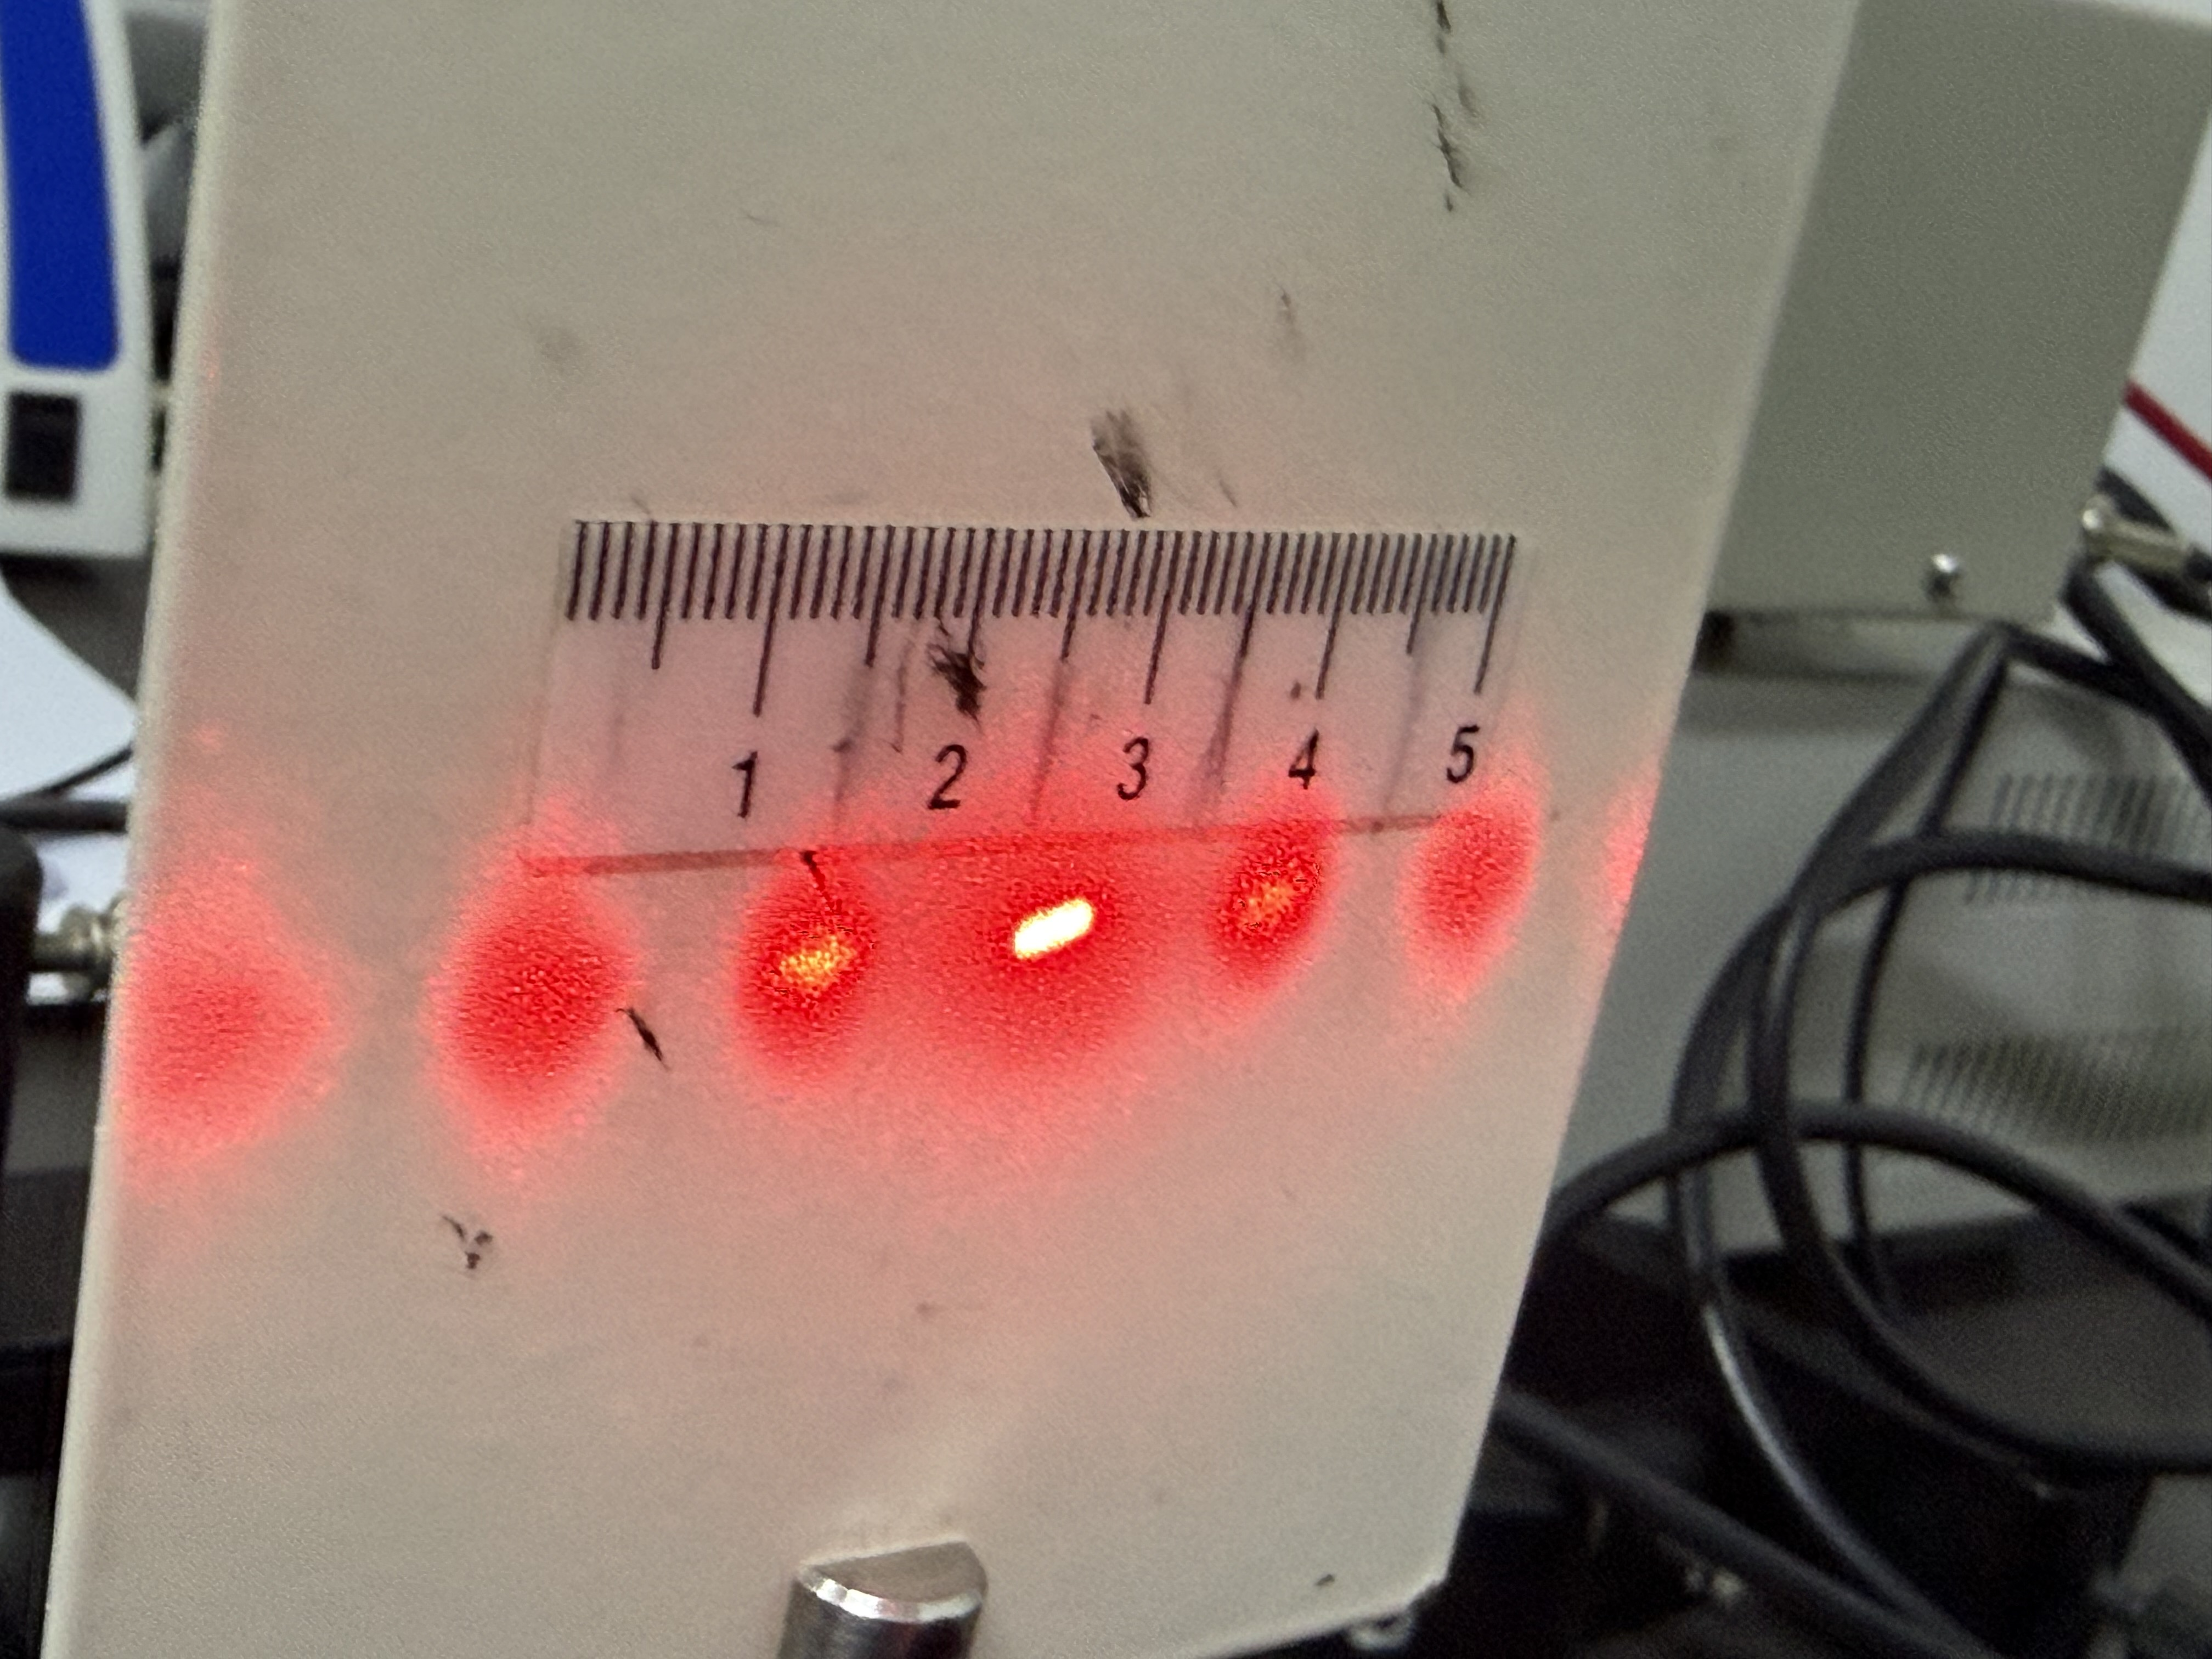
\includegraphics[width=\textwidth,height=6cm]{dot}
            \caption{衍射光斑的测量}
            \label{key}
        \end{subfigure}
        \hfill
        \begin{subfigure}{0.47\textwidth}
            \includegraphics[width=\textwidth,height=6cm]{sub}
            \caption{显微镜下观察到的液晶}
            \label{key}
        \end{subfigure}
        \caption{液晶衍射实验}
        \label{key}
    \end{figure}

    \section{总结}
        在无液晶的情况下，入射光通过起偏器和检偏器后仍为线偏振光。通过测量光强的极大值和极小值，可以计算光的线偏度 $L_0 = I_{\text{max}}/I_{\text{min}}$。光强的极值反映了入射光的线偏振程度，实验中线偏度有限主要是由于仪器散射、背景光干扰以及偏振片的非理想特性。

将液晶盒放入光路后，出射光的消光位置出现规律变化，由两次消光角度差可计算液晶盒的旋光角 $\beta = |\theta_i - \theta_j|$。进一步旋转液晶盒时，出射光的极值角度随液晶盒角度变化，反映液晶的附加相位差 $\delta = (2\pi/\lambda)(n_o - n_e)d$，其中 $n_o$ 和 $n_e$ 分别为普通光和非常光折射率，$d$ 为光在液晶层中的传播长度。液晶盒的旋光性来源于分子在盒内均匀扭曲排列，使左旋光和右旋光折射率不同，从而使线偏振光的振动面旋转。双折射效应是由于液晶分子排列的各向异性，使不同偏振分量经历不同光程，产生相位差。两种效应叠加后，出射光偏振状态随液晶盒旋转而变化。

在常黑模式下施加三角波驱动电压，可记录液晶盒的电光响应曲线，并定义阈值电压 $V_{\text{th}}$、饱和电压 $V_s$ 以及阈值锐度 $\gamma$。阈值电压对应液晶分子开始响应电场的最小电压，饱和电压表示液晶分子完全沿电场方向排列时光学透过率达到稳定值，阈值锐度反映液晶光学响应随电压变化的陡峭程度。这些现象的出现主要源于液晶的介电各向异性：外加电场改变分子排列，从而调制液晶盒的旋光和双折射性质。

利用方波脉冲驱动液晶盒，可以测量上升沿时间 $T_{\text{on}}$ 和下降沿时间 $T_{\text{off}}$，分别对应液晶分子从初始排列响应到电场方向排列，以及电场撤去后恢复到初始排列的时间。响应时间受液晶黏度、分子长径比和液晶层厚度影响，因此上升沿和下降沿时间可能存在差异，体现液晶分子动力学的滞后性。

当施加低频电压超过一定阈值时，液晶内部带电杂质引起分子环流，形成周期性折射率变化，在屏上出现衍射图样。通过测量衍射光斑间距，可利用公式 $d \approx \lambda/\sin\theta \approx \lambda/(x/r)$ 估算液晶形成的光栅常数。衍射现象的出现和消失随电压变化，说明液晶分子环流的形成和消散，这验证了液晶在电场作用下可形成空间周期性结构，从而调制光的传播。

综合实验观察可知，液晶盒具有明显的旋光和双折射效应，这是由液晶分子的各向异性排列导致的。电光响应曲线反映液晶分子对外加电场的敏感性，阈值电压和饱和电压展示分子排列的可调范围。电光响应时间揭示液晶分子的动力学特性，上升沿和下降沿时间的差异体现分子排列的滞后性。衍射现象说明液晶在电场作用下可形成空间周期性结构，并可用于估算光栅常数，从而进一步验证液晶的电光和光学各向异性性质。
\begin{thebibliography}{99}
        \bibitem{1}
        北京师范大学物理实验教学中心. 近代物理实验讲义一 (2019)
    \end{thebibliography}

    
\end{document}